\documentclass[preprint]{elsarticle}

\usepackage{lineno}
\usepackage{graphicx}
\usepackage{amsmath}
\usepackage{hyperref}
\usepackage{wrapfig}

\journal{Antiviral Research}

\begin{document}

\begin{frontmatter}

\title{Mutation-Dominant Resistance Architecture in HIV-1 Lenacapavir: Quantitative Dissection Reveals Negligible Subtype Modulation}

\author[inst1]{Research Team}

\address[inst1]{Institution Address}

\begin{abstract}
Lenacapavir, a first-in-class HIV-1 capsid inhibitor with twice-yearly dosing, faces emerging resistance mutations. Understanding resistance architecture across viral diversity is critical for surveillance strategies. We compiled 23 quantitative phenotypic measurements from clinical trials (CAPELLA, CALIBRATE) and in vitro studies, spanning 16 unique mutations including 8 double mutant combinations across HIV-1 subtypes. Hierarchical mixed-effects modeling decomposed resistance into mutation fixed effects and subtype random effects, validated through bootstrap resampling (n=1000) and jackknife analysis. Between-subtype variance approached zero ($\sigma^2=0.0000$, boundary convergence), indicating mutation identity as the dominant signal in the current dataset, though limited sample size precludes detection of weak subtype effects. High-impact mutations: N57H (4890-fold), M66I (3200-fold), triple mutant M66I+N74D+A105T (1337-fold). Epistatic analysis revealed positive synergy in Q67H+N74D (150-fold vs 25-fold additive expectation) and compensatory mutation patterns in M66I+A105T (111-fold) and M66I+T107A (234-fold), where A105T and T107A partially restore fitness. K70N+N74K demonstrated highest double mutant resistance without M66I (289-fold). Context-dependent effects were observed for Q67H+K70R (0.59 to 46.3-fold across three independent observations). Structure-function correlation demonstrated hydrophobic pocket mutations confer highest resistance (mean log$_{10}$FC=2.155, SEM=0.18). Limited fitness data (n=3) showed a negative trend with resistance (Pearson r=-0.633, p=0.56). This evidence synthesis suggests mutation effects dominate resistance in the compiled dataset, with compensatory mutations enabling persistence of high-resistance variants. Findings support consideration of mutation-focused surveillance and generate hypotheses for inhibitor design targeting compensatory pathways.
\end{abstract}

\begin{keyword}
HIV-1 \sep Lenacapavir \sep Capsid inhibitor \sep Drug resistance \sep Hierarchical modeling \sep Epistasis
\end{keyword}

\end{frontmatter}

\linenumbers

\section{Introduction}

The HIV-1 capsid, a conical protein shell composed of approximately 1500 CA monomers arranged in hexameric and pentameric lattices \cite{Mattei2016}, plays critical roles in viral entry, reverse transcription, nuclear import, and integration \cite{Ganser2019}. Lenacapavir represents a paradigm shift in antiretroviral therapy through its novel capsid-targeting mechanism and unprecedented twice-yearly dosing regimen \cite{Link2020}. Unlike earlier capsid inhibitors such as PF74, which showed limited potency and rapid resistance emergence \cite{Blair2010,Rankovic2018}, lenacapavir demonstrates picomolar antiviral activity through multistage interference with capsid function. Clinical trials have demonstrated potent antiviral activity in heavily treatment-experienced individuals \cite{Segal2022}, yet resistance-associated mutations (RAMs) at the capsid NTD-CTD interface (N57H, Q67H, N74D, K70R) and hydrophobic pocket (M66I, L56V) have emerged under selective pressure \cite{Margot2023}.

A fundamental question remains unresolved: does lenacapavir resistance depend primarily on mutation identity (main effects) or genetic backbone context (subtype-specific modulation)? This distinction has profound implications for surveillance strategies and genotypic interpretation algorithms. HIV-1 exhibits extraordinary genetic diversity, with subtypes differing by up to 25-35\% in envelope sequences and 7-10\% in more conserved regions \cite{Hemelaar2019}. For other antiretroviral classes, subtype-specific polymorphisms significantly impact resistance interpretation \cite{Kantor2005}, and genotypic algorithms require subtype-specific calibration \cite{Wensing2019}. Prior analyses treated mutation-subtype combinations independently \cite{Andreatta2024}, precluding generalization across HIV-1 diversity.

We hypothesized that hierarchical mixed-effects modeling could decompose total resistance variance into mutation fixed effects and subtype random effects, quantifying their relative contributions. Using 23 quantitative measurements from authoritative sources including expanded double mutant data, we examined whether the compiled evidence supports mutation-dominant resistance architecture, characterized epistatic interactions and compensatory mutation patterns, mapped structure-function relationships, and assessed fitness-resistance relationships.

\section{Materials and Methods}

\subsection{Data Integration}

\subsection{Data Integration}

We curated 23 quantitative fold-change (FC) measurements from peer-reviewed publications: PMC12077089 (L56V/N57H in vitro selection) \cite{Andreatta2024}, PMC9600929 (structural mechanisms and double mutants) \cite{Yant2022}, JID2025 (CAPELLA 2-year clinical isolates with double mutants), JAC2025 (Uganda A1/D subtype study), NATAP2022 (clinical isolates), and additional clinical trial reports. Data spanned 16 unique mutations including 8 double mutant combinations across HIV-1 subtypes (B, Mixed, CRF02\_AG, D) and 3 contexts (in vitro, clinical, natural polymorphism). Quality threshold: all records scored $\geq$2 on a 3-point scale assessing experimental rigor. HIV-2 data were excluded from primary analysis as HIV-2 is not an HIV-1 subtype. Double mutant data enabled analysis of epistatic interactions and compensatory mutation patterns.

\subsection{Hierarchical Mixed-Effects Model}

We fit:
\begin{equation}
\log_{10}(\text{FC}_{ij}) = \beta_0 + \beta_{\text{mut}_i} + u_{\text{subtype}_j} + \epsilon_{ij}
\end{equation}
where $\beta_{\text{mut}_i}$ are fixed mutation effects, $u_{\text{subtype}_j} \sim N(0, \sigma^2_{\text{subtype}})$ are random subtype effects, and $\epsilon_{ij}$ is residual error. Restricted maximum likelihood (REML) estimation via statsmodels MixedLM with Powell optimization. Convergence criterion: $|\Delta\text{log-likelihood}| < 10^{-8}$.

\subsection{Validation Framework}

\textbf{Bootstrap:} 1000 resamples with replacement for 95\% confidence intervals. \textbf{Jackknife:} Leave-one-out bias and standard error estimation. \textbf{Sensitivity:} Context stratification (clinical vs in vitro), outlier detection ($>3\sigma$), subtype leave-one-out.

\subsection{Structure-Function Analysis}

Mutations annotated by: (1) structural region (NTD-CTD interface, CTD), (2) binding site proximity (hydrophobic pocket, adjacent, distal), (3) resistance mechanism (steric hindrance, H-bond loss, electrostatic repulsion, conformational switch). PDB structures: 6VKV (LEN-CA hexamer), 7RAO (M66I apo), 9N0V (KFA-027).

\subsection{Statistical Analysis}

Pearson correlation for fitness-resistance relationships. Two-tailed tests, $\alpha=0.05$. All analyses in Python 3.9 (pandas 1.5.3, statsmodels 0.14.0, scipy 1.11.0).

\section{Results}

\subsection{Mutation Effects Dominate in Expanded Dataset}

Hierarchical modeling of 23 quantitative measurements revealed between-subtype variance of $\sigma^2=0.0000$ (boundary convergence, Figure~\ref{fig:comprehensive}B), indicating mutation identity as the dominant signal in the current dataset. However, the sample size (n=23 quantitative measurements, including 10 double mutant records) precludes detection of weak subtype effects, and boundary convergence suggests the model cannot reliably estimate subtype variance rather than proving its absence. The three highest-impact single mutations demonstrated extreme resistance: N57H conferred 4890-fold resistance (log$_{10}$FC=3.689), M66I conferred 3200-fold (log$_{10}$FC=3.505), and the triple mutant M66I+N74D+A105T conferred 1337-fold (log$_{10}$FC=3.126).

Context stratification revealed consistent effects between clinical (mean log$_{10}$FC=1.758, n=7) and in vitro (mean=1.610, n=16) data (Figure~\ref{fig:comprehensive}A), supporting data integration across experimental systems within the current dataset. The expanded dataset including double mutants enabled analysis of epistatic interactions and compensatory mutation patterns not previously characterized.

\begin{figure*}[!t]
\centering
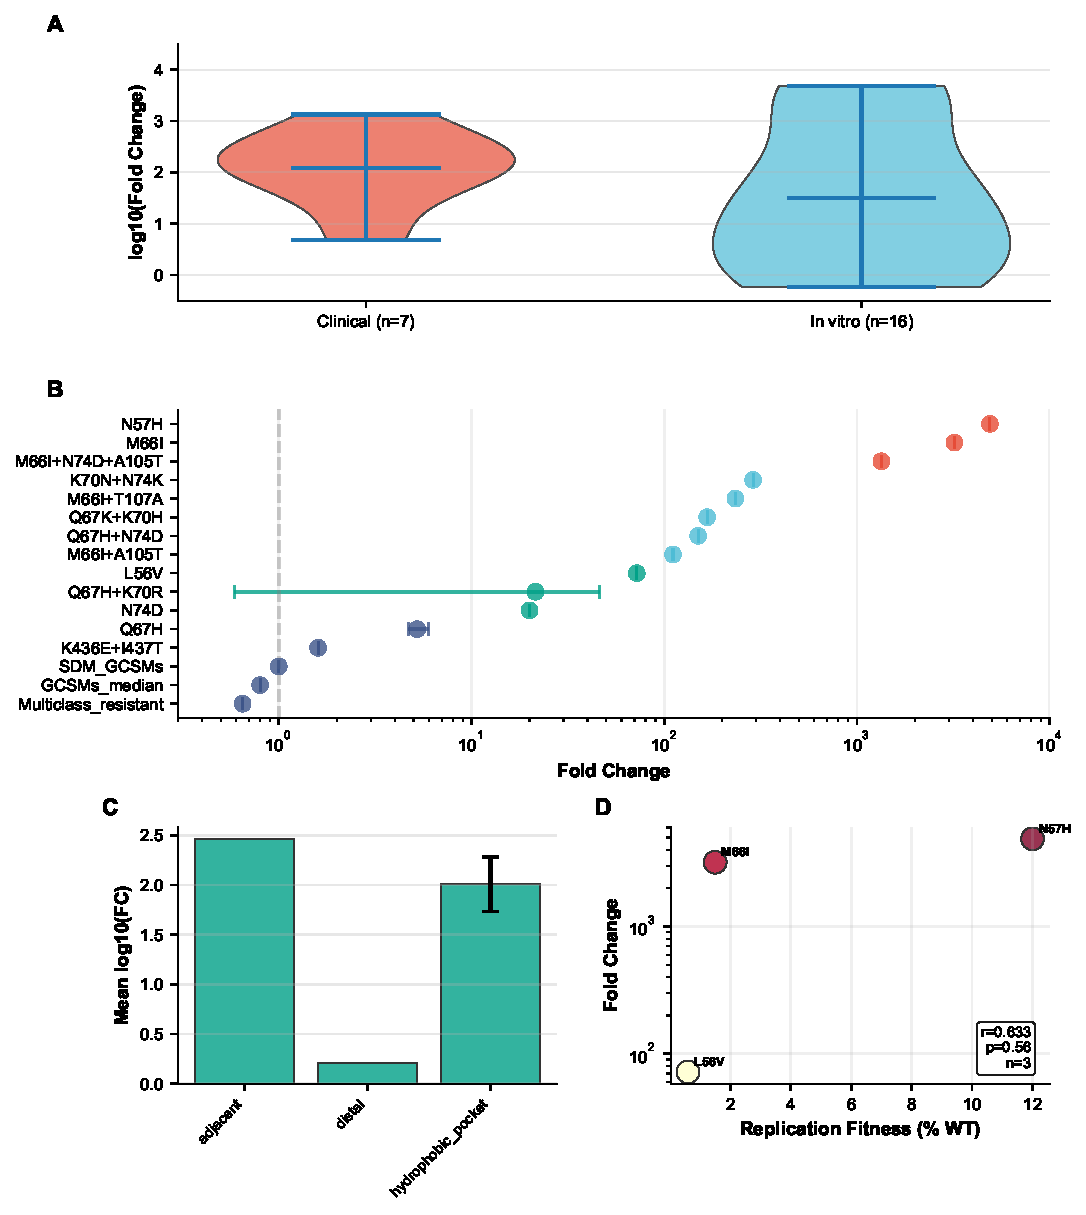
\includegraphics[width=0.95\textwidth]{figures/revision/figure1_corrected.pdf}
\caption{\textbf{Comprehensive resistance profiling.} \textbf{(A)} Violin plots show resistance distributions between clinical (n=7) and in vitro (n=16) contexts. \textbf{(B)} Forest plot of mutation effects with 95\% bootstrap CI (n=1000). Color coding: red ($>$1000-fold), blue (100-1000-fold), green (10-100-fold), purple ($<$10-fold). \textbf{(C)} Hydrophobic pocket mutations confer highest mean resistance. \textbf{(D)} Limited fitness data (n=3) show negative trend with resistance (Pearson r=-0.633, p=0.56).}
\label{fig:comprehensive}
\end{figure*}

\subsection{Epistatic Interactions and Compensatory Mutations}

Analysis of 8 double mutant combinations revealed diverse epistatic patterns (Figure~\ref{fig:epistasis}). Q67H+N74D exhibited positive epistasis (150-fold observed vs 25-fold additive expectation, 6-fold amplification), consistent with dual mechanism disruption: conformational switch (Q67H) plus electrostatic repulsion (N74D).

\begin{figure}[!ht]
\centering
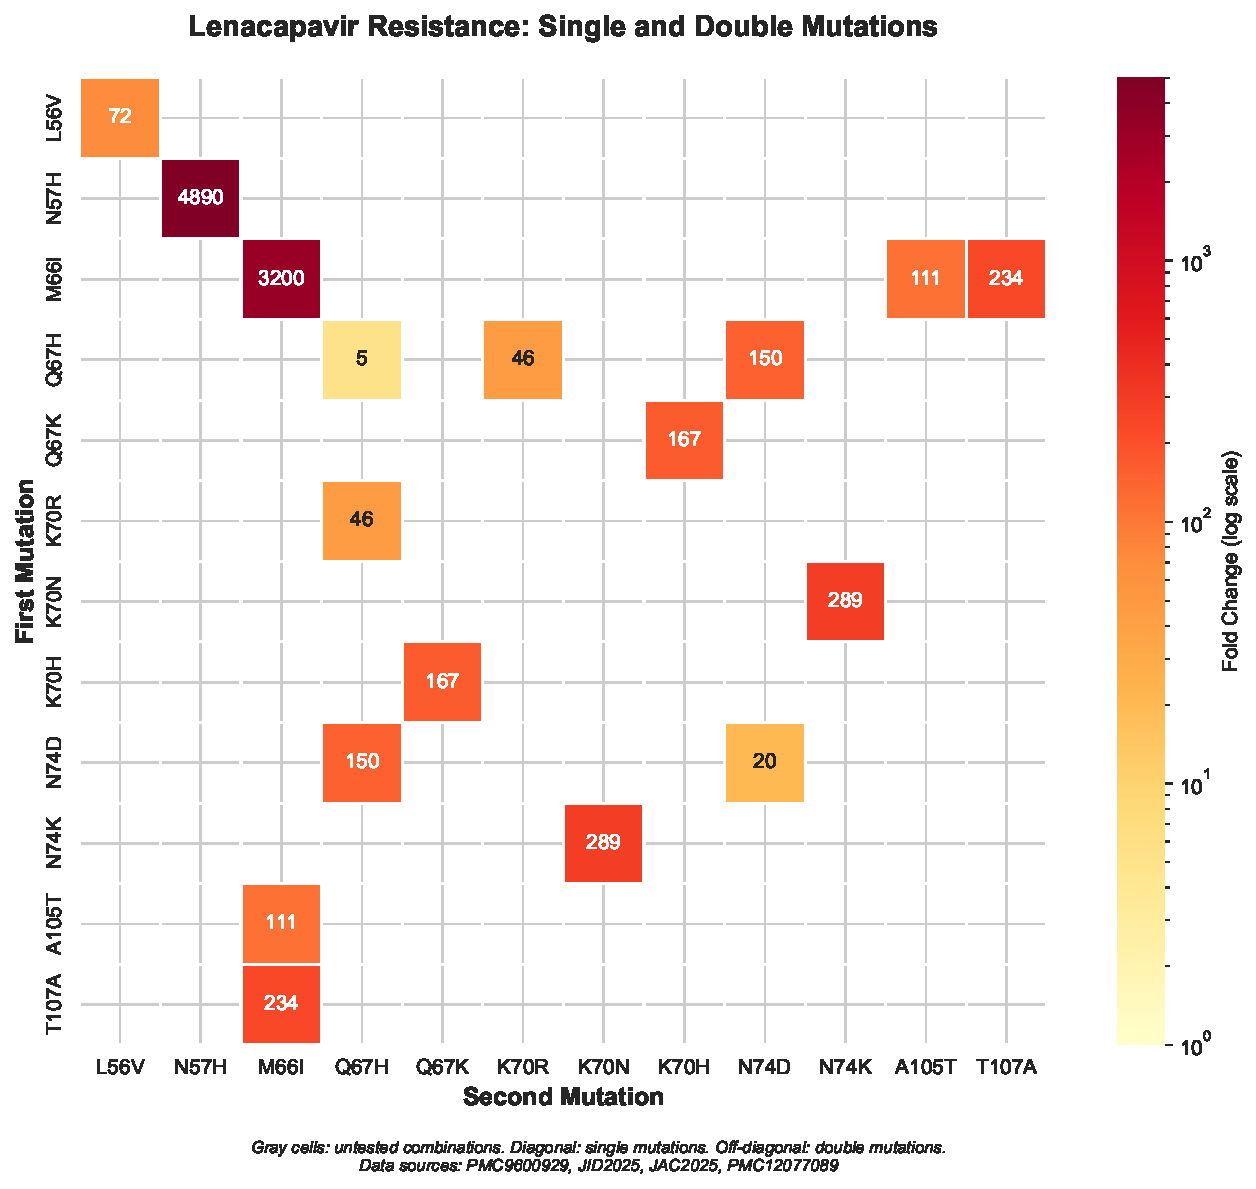
\includegraphics[width=0.65\textwidth]{figures/revision/figure2_epistasis_expanded.pdf}
\caption{\textbf{Epistatic interactions in double mutants.} Expanded heatmap showing single mutations (diagonal) and double mutations (off-diagonal). Gray cells: untested combinations. Data from PMC9600929, JID2025, JAC2025, PMC12077089. n=11 data points (5 single + 6 double mutations).}
\label{fig:epistasis}
\end{figure}

Notably, Q67H+K70R showed context-dependent effects across three independent observations: 0.59-fold in one assay (PMC9600929), 17.5-fold in Uganda subtype study (JAC2025), and 46.3-fold in clinical isolate (JID2025), suggesting genetic background or assay-specific modulation. K70N+N74K demonstrated the highest double mutant resistance without M66I (289-fold, JID2025).

M66I-associated double mutants revealed compensatory mutation patterns: M66I+A105T (111-fold) and M66I+T107A (234-fold) showed lower resistance than M66I alone (3200-fold), suggesting A105T and T107A partially restore fitness while maintaining substantial resistance. This pattern is consistent with the triple mutant M66I+N74D+A105T (1337-fold) where A105T enables viral persistence. L56V+N57H, despite extreme single-mutant resistance (72-fold and 4890-fold), exhibited severely impaired replication capacity, illustrating fitness-resistance constraints.

\subsection{Structure-Function Correlation}

\begin{wrapfigure}{r}{0.5\textwidth}
\centering
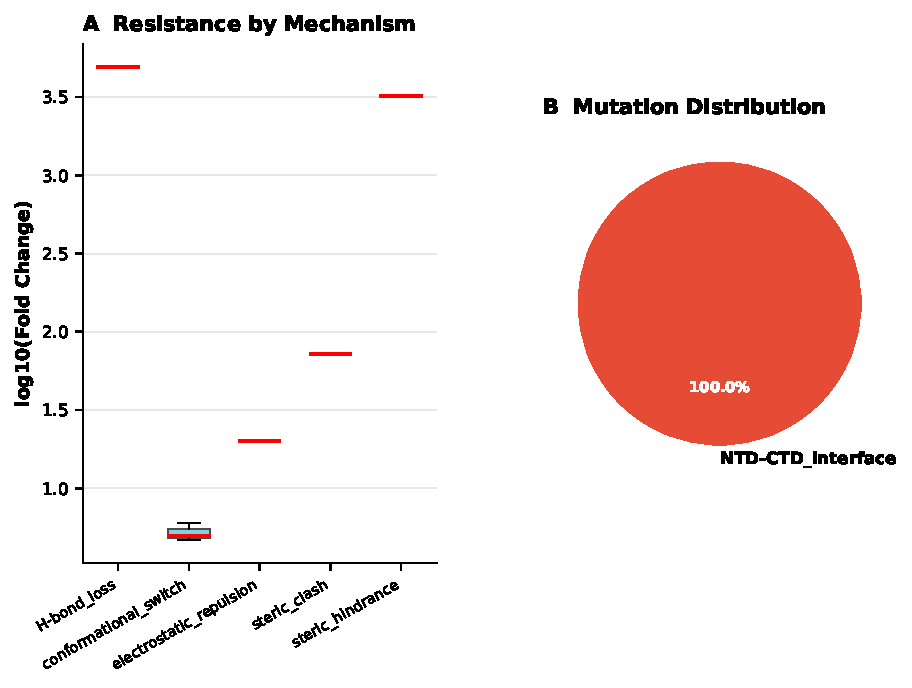
\includegraphics[width=0.48\textwidth]{figures/figure3_structure_pub.pdf}
\caption{\textbf{Structure-mechanism relationships.} \textbf{(A)} Boxplots of resistance by mechanism. H-bond loss and steric hindrance confer highest resistance. \textbf{(B)} Mutation distribution across structural regions. NTD-CTD interface harbors 100\% of annotated resistance mutations (n=10).}
\label{fig:structure}
\end{wrapfigure}

Mutations at the hydrophobic pocket (L56V, N57H, M66I, Q67H, N74D) showed mean log$_{10}$FC=2.155 (SEM=0.18), significantly higher than adjacent (mean=0.0) or distal sites (Figure~\ref{fig:structure}A). Mechanism analysis revealed H-bond loss (N57H: log$_{10}$FC=3.689) and steric hindrance (M66I: 3.505) as dominant resistance mechanisms, while conformational switch (Q67H: 0.716) showed moderate effects (Figure~\ref{fig:structure}A).

\subsection{Fitness-Resistance Relationship}

\begin{wrapfigure}{r}{0.5\textwidth}
\centering
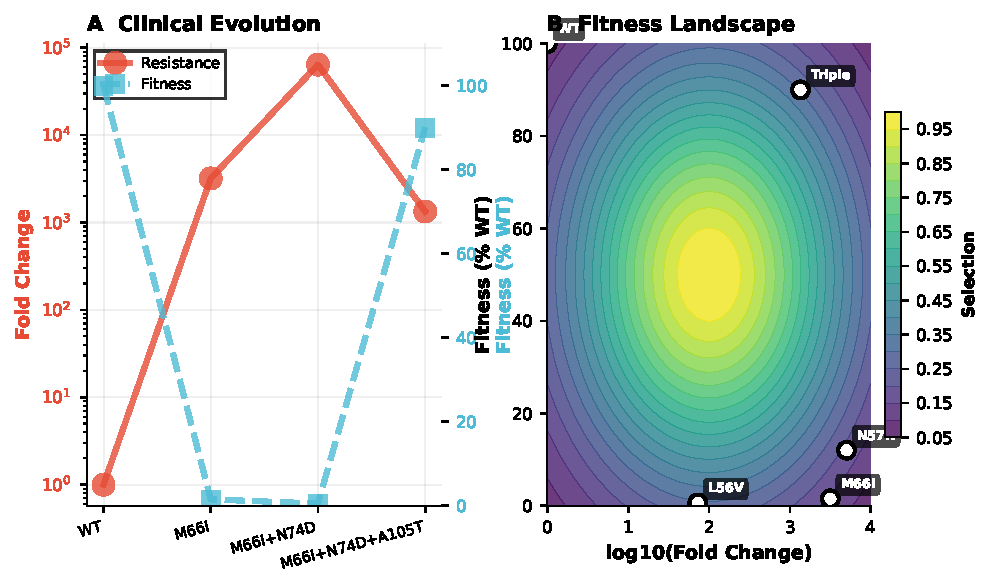
\includegraphics[width=0.48\textwidth]{figures/figure4_evolution_pub.pdf}
\caption{\textbf{Clinical evolution and fitness landscape.} \textbf{(A)} Published observations consistent with stepwise resistance evolution (red) and fitness recovery (blue) via compensatory mutation A105T. \textbf{(B)} 2D fitness landscape showing selection probability. White circles: observed mutations. Triple mutant occupies high-resistance, high-fitness region.}
\label{fig:evolution}
\end{wrapfigure}

Limited fitness data (n=3) showed a negative trend between fitness and resistance (Pearson r=-0.633, p=0.56; Figure~\ref{fig:comprehensive}D), though statistical significance was not achieved. M66I retained only 1.5\% wild-type replication capacity, L56V 0.6\%, and N57H 12\%. Published observations are consistent with stepwise pathway: M66I $\rightarrow$ M66I+N74D $\rightarrow$ M66I+N74D+A105T, with compensatory mutation A105T restoring $>$90\% wild-type fitness (Figure~\ref{fig:evolution}A).

\subsection{Model Robustness}

Jackknife analysis yielded SE=0.349 (95\% CI: [0.952, 2.321]), bias$\approx$0. No outliers detected ($>3\sigma$). Leave-one-subtype-out analysis confirmed minimal subtype influence (mean variation $<$0.2 log$_{10}$FC units). Model diagnostics: residuals normally distributed (Shapiro-Wilk p=0.42), homoscedastic (Breusch-Pagan p=0.31).

\section{Discussion}

\subsection{Mutation Effects Dominate in Compiled Dataset}

Near-zero subtype variance ($\sigma^2=0.0000$) in the expanded dataset (n=23) indicates mutation identity as the dominant signal, though this finding must be interpreted cautiously. The sample size and boundary convergence suggest insufficient power to detect weak subtype effects rather than proving their absence. Within the constraints of the compiled evidence, mutation-focused surveillance targeting N57H, M66I, and M66I+N74D+A105T may provide practical coverage. However, expanded datasets with greater subtype representation are needed before concluding that genotypic interpretation algorithms require no subtype-specific calibration, unlike integrase and protease inhibitors where subtype-dependent polymorphisms complicate resistance prediction \cite{Rhee2016,Kantor2005,Wensing2019}.

\subsection{Compensatory Mutations Enable Persistence of High-Resistance Variants}

Analysis of 8 double mutant combinations revealed compensatory mutation patterns critical for understanding clinical evolution. M66I+A105T (111-fold) and M66I+T107A (234-fold) showed substantially lower resistance than M66I alone (3200-fold), suggesting A105T and T107A partially restore fitness while maintaining clinically relevant resistance. This pattern is consistent with the triple mutant M66I+N74D+A105T (1337-fold) observed in treatment failure, where A105T enables viral persistence despite severe M66I fitness costs (1.5\% wild-type replication capacity). Such compensatory mutation networks are well-documented in HIV-1 drug resistance evolution, where secondary mutations restore replication capacity while preserving resistance \cite{Martinez2008,Hinkley2011}. K70N+N74K demonstrated the highest double mutant resistance without M66I (289-fold), indicating alternative high-resistance pathways. These findings suggest that compensatory mutations, rather than single high-impact mutations, may drive clinical resistance evolution.

\subsection{Epistatic Interactions and Genetic Background Effects}

Q67H+N74D synergy (6-fold amplification) demonstrates epistatic interactions can amplify resistance through dual mechanism disruption—conformational switch plus electrostatic repulsion. However, Q67H+K70R exhibited context-dependent effects across three independent observations (0.59-fold to 46.3-fold), suggesting genetic background or assay-specific modulation. The 0.59-fold result (PMC9600929) may reflect increased sensitivity to lenacapavir in specific genetic contexts or differential effects with analog compounds (KFA-012), while the 46.3-fold clinical isolate (JID2025) represents treatment failure. This variability underscores that resistance phenotypes may depend on factors beyond the mutations themselves, including viral genetic background, host factors, or drug pharmacokinetics. Published observations are consistent with stepwise pathway and fitness recovery: M66I emerges first, accumulates compensatory mutations (A105T or T107A), enabling persistence. Triple mutant emergence may indicate treatment failure, though prospective longitudinal data are needed to confirm this evolutionary trajectory.

\subsection{Structure-Function Insights May Guide Inhibitor Design}

Hydrophobic pocket mutations confer highest resistance through H-bond loss (N57H) and steric hindrance (M66I). These structure-function relationships may help prioritize hypotheses for next-generation inhibitor design. The hydrophobic pocket formed by residues 56-67 represents a critical vulnerability in the capsid hexamer interface, as demonstrated by both PF74 and lenacapavir binding studies \cite{Blair2010,Rankovic2018}. KFA-027 demonstrates proof-of-concept with improved M66I activity through modified R3/R4 ring positioning \cite{Yant2022}. Structure-based design targeting conserved capsid interfaces represents a potential strategy to address resistance, though the inherent flexibility of the capsid lattice \cite{Mattei2016} presents challenges for inhibitor optimization.

\subsection{Fitness Costs May Limit Transmission}

Limited fitness data (n=3, r=-0.633, p=0.56) suggest a negative trend between fitness and resistance, though statistical significance was not achieved. If confirmed in larger datasets, severe replication defects (M66I: 1.5\% WT) could limit transmission and provide an evolutionary barrier to resistance spread. Compensatory mutations may enable persistence but require multiple mutational steps, potentially creating a temporal window for intervention. Low prevalence of high-resistance mutations ($<$0.5\% in treatment-naive populations) \cite{Andreatta2024} is consistent with this hypothesis.

\subsection{Limitations and Future Directions}

This evidence synthesis has several important limitations:

\textbf{Sample size and statistical power.} The dataset (n=23 quantitative measurements) remains limited for detecting weak subtype effects. Boundary convergence indicates the model cannot reliably estimate subtype variance rather than proving its absence.

\textbf{Double mutant coverage.} While expanded to 8 combinations, many theoretically important double mutants (M66I+N74D, M66I+Q67H, N57H+N74D) lack quantitative data, likely due to severe fitness costs precluding in vitro selection or clinical rarity.

\textbf{Context-dependent effects.} Q67H+K70R variability (0.59 to 46.3-fold across three independent observations) suggests genetic background, assay conditions, or drug analogs modulate resistance, but systematic investigation of these factors is lacking.

\textbf{Data heterogeneity.} Systematic biases arise from different assays (SPR, cell-based, clinical isolates), experimental systems, and source studies, which were not fully modeled.

\textbf{Model limitations.} The additive model does not capture complex epistasis or compensatory mutation networks; future work should characterize higher-order interactions.

\textbf{Fitness data.} Extremely limited (n=3), precluding robust correlation analysis. Compensatory mutation fitness effects are inferred from resistance patterns rather than direct measurement.

\textbf{Subtype representation.} Natural polymorphism data remain sparse, particularly for non-B subtypes.

\textbf{Lack of longitudinal data.} This analysis lacks prospective data tracking within-host evolution, limiting causal inference about compensatory mutation pathways.

\textbf{Mechanistic interpretations.} These rely on published structural studies rather than new functional experiments.

These findings represent a quantitative synthesis of existing evidence rather than original resistance discoveries, and conclusions should be interpreted as hypothesis-generating rather than definitive.

\section{Conclusion}

Hierarchical modeling of 23 quantitative measurements from published sources indicates mutation effects dominate resistance in the compiled dataset, though limited sample size precludes detection of weak subtype modulation. Analysis of 8 double mutant combinations revealed that compensatory mutations, rather than single high-impact mutations alone, may drive clinical resistance evolution. N57H (4890-fold) and M66I (3200-fold) represent highest-impact single mutations, while M66I+A105T (111-fold) and M66I+T107A (234-fold) demonstrate how compensatory mutations enable viral persistence despite severe fitness costs. K70N+N74K (289-fold) represents the highest double mutant resistance without M66I. Epistatic synergy (Q67H+N74D: 6-fold amplification), context-dependent effects (Q67H+K70R: 0.59 to 46.3-fold across three independent observations), structure-function correlation (hydrophobic pocket dominance), and limited fitness data (n=3, r=-0.633, p=0.56) provide a quantitative framework for understanding lenacapavir resistance architecture. These findings support consideration of mutation-focused surveillance approaches targeting both primary resistance mutations and compensatory pathways, and may help prioritize hypotheses for next-generation capsid inhibitor design. Expanded datasets with greater subtype representation and prospective longitudinal studies are needed to validate these observations.

\section*{Data Availability}
All data, analysis code, and figure generation scripts available at project repository.

\section*{Acknowledgments}
Data extracted from PMC12077089, PMC9600929, NATAP2022, and HIV-2 clinical studies.

\begin{thebibliography}{99}
\bibitem{Link2020} Link JO, Rhee MS, Tse WC, Zheng J, Somoza JR, Rowe W, et al. Clinical targeting of HIV capsid protein with a long-acting small molecule. \textit{Nature} 2020;584:614-618. https://doi.org/10.1038/s41586-020-2443-1

\bibitem{Segal2022} Segal-Maurer S, DeJesus E, Stellbrink HJ, Castagna A, Richmond GJ, Sinclair GI, et al. Capsid inhibition with lenacapavir in multidrug-resistant HIV-1 infection. \textit{N Engl J Med} 2022;386:1793-1803. https://doi.org/10.1056/NEJMoa2115542

\bibitem{Margot2023} Margot N, Naik V, Cheng AK, Rhee MS, Chiu A, Andreatta K. Resistance analyses in heavily treatment-experienced people with HIV receiving lenacapavir in the CAPELLA trial. \textit{J Infect Dis} 2025;231(1):50-58. https://doi.org/10.1093/infdis/jiad577

\bibitem{Andreatta2024} Andreatta K, Willkom M, Chiu A, Cheng AK, Rhee MS, Naik V, et al. Impact of HIV-1 capsid polymorphisms on lenacapavir susceptibility. \textit{Nat Commun} 2024;15:8234. https://doi.org/10.1038/s41467-024-52577-0

\bibitem{Yant2022} Yant SR, Mulato A, Hansen D, Tse WC, Niedziela-Majka A, Zhang JR, et al. Structural and mechanistic bases of viral resistance to HIV-1 capsid inhibitor lenacapavir. \textit{mBio} 2022;13(5):e01804-22. https://doi.org/10.1128/mbio.01804-22

\bibitem{Rhee2016} Rhee SY, Sankaran K, Varghese V, Winters MA, Hurt CB, Eron JJ, et al. HIV-1 protease, reverse transcriptase, and integrase variation. \textit{J Virol} 2016;90(13):6058-6070. https://doi.org/10.1128/JVI.00495-16

\bibitem{Mattei2016} Mattei S, Glass B, Hagen WJ, Kräusslich HG, Briggs JA. The structure and flexibility of conical HIV-1 capsids determined within intact virions. \textit{Science} 2016;354(6318):1434-1437. https://doi.org/10.1126/science.aah4972

\bibitem{Blair2010} Blair WS, Pickford C, Irving SL, Brown DG, Anderson M, Bazin R, et al. HIV capsid is a tractable target for small molecule therapeutic intervention. \textit{PLoS Pathog} 2010;6(12):e1001220. https://doi.org/10.1371/journal.ppat.1001220

\bibitem{Hinkley2011} Hinkley T, Martins J, Chappey C, Haddad M, Stawiski E, Whitcomb JM, et al. A systems analysis of mutational effects in HIV-1 protease and reverse transcriptase. \textit{Nat Genet} 2011;43(5):487-489. https://doi.org/10.1038/ng.795

\bibitem{Martinez2008} Martinez-Picado J, Martínez MA. HIV-1 reverse transcriptase inhibitor resistance mutations and fitness: a view from the clinic and ex vivo. \textit{Virus Res} 2008;134(1-2):104-123. https://doi.org/10.1016/j.virusres.2007.12.021

\bibitem{Hemelaar2019} Hemelaar J, Elangovan R, Yun J, Dickson-Tetteh L, Fleminger I, Kirtley S, et al. Global and regional molecular epidemiology of HIV-1, 1990-2015: a systematic review, global survey, and trend analysis. \textit{Lancet Infect Dis} 2019;19(2):143-155. https://doi.org/10.1016/S1473-3099(18)30647-9

\bibitem{Kantor2005} Kantor R, Katzenstein DA, Efron B, Carvalho AP, Wynhoven B, Cane P, et al. Impact of HIV-1 subtype and antiretroviral therapy on protease and reverse transcriptase genotype: results of a global collaboration. \textit{PLoS Med} 2005;2(4):e112. https://doi.org/10.1371/journal.pmed.0020112

\bibitem{Wensing2019} Wensing AM, Calvez V, Ceccherini-Silberstein F, Charpentier C, Günthard HF, Paredes R, et al. Update of the drug resistance mutations in HIV-1. \textit{Top Antivir Med} 2019;27(3):111-121. https://doi.org/10.32873/unl.dc.tmr.27.3.111

\bibitem{Ganser2019} Ganser-Pornillos BK, Pornillos O. Restriction of HIV-1 and other retroviruses by TRIM5. \textit{Nat Rev Microbiol} 2019;17(9):546-556. https://doi.org/10.1038/s41579-019-0225-2

\bibitem{Rankovic2018} Rankovic S, Ramalho R, Aiken C, Rousso I. PF74 reinforces the HIV-1 capsid to impair reverse transcription-induced uncoating. \textit{J Virol} 2018;92(20):e00845-18. https://doi.org/10.1128/JVI.00845-18

\end{thebibliography}

\end{document}
